\documentclass[aspectratio=169]{../latex_main/tntbeamer}  % you can pass all options of the beamer class, e.g., 'handout' or 'aspectratio=43'
\usepackage{dsfont}
\usepackage{bm}
\usepackage[english]{babel}
\usepackage[T1]{fontenc}
%\usepackage[utf8]{inputenc}
\usepackage{graphicx}
\graphicspath{ {./figures/} }
\usepackage{algorithm}
\usepackage[ruled,vlined,algo2e,linesnumbered]{algorithm2e}
\usepackage{hyperref}
\usepackage{booktabs}
\usepackage{mathtools}

\usepackage{amsmath,amssymb}

\DeclareMathOperator*{\argmax}{arg\,max}
\DeclareMathOperator*{\argmin}{arg\,min}

\usepackage{amsbsy}
\newcommand{\vect}[1]{\bm{#1}}
%\newcommand{\vect}[1]{\boldsymbol{#1}}

\usepackage{pgfplots}
\pgfplotsset{compat=1.16}
\usepackage{tikz}
\usetikzlibrary{trees} 
\usetikzlibrary{shapes.geometric}
\usetikzlibrary{positioning,shapes,shadows,arrows,calc,mindmap}
\usetikzlibrary{positioning,fadings,through}
\usetikzlibrary{decorations.pathreplacing}
\usetikzlibrary{intersections}
\pgfdeclarelayer{background}
\pgfdeclarelayer{foreground}
\pgfsetlayers{background,main,foreground}
\tikzstyle{activity}=[rectangle, draw=black, rounded corners, text centered, text width=8em]
\tikzstyle{data}=[rectangle, draw=black, text centered, text width=8em]
\tikzstyle{myarrow}=[->, thick, draw=black]

% Define the layers to draw the diagram
\pgfdeclarelayer{background}
\pgfdeclarelayer{foreground}
\pgfsetlayers{background,main,foreground}

% Requires XeLaTeX or LuaLaTeX
%\usepackage{unicode-math}

\usepackage{fontspec}
%\setsansfont{Arial}
\setsansfont{RotisSansSerifStd}[ 
Path=../latex_main/fonts/,
Extension = .otf,
UprightFont = *-Regular,  % or *-Light
BoldFont = *-ExtraBold,  % or *-Bold
ItalicFont = *-Italic
]
\setmonofont{Cascadia Mono}[
Scale=0.8
]

% scale factor adapted; mathrm font added (Benjamin Spitschan @TNT, 2021-06-01)
%\setmathfont[Scale=1.05]{Libertinus Math}
%\setmathrm[Scale=1.05]{Libertinus Math}

% other available math fonts are (not exhaustive)
% Latin Modern Math
% XITS Math
% Libertinus Math
% Asana Math
% Fira Math
% TeX Gyre Pagella Math
% TeX Gyre Bonum Math
% TeX Gyre Schola Math
% TeX Gyre Termes Math

% Literature References
\newcommand{\lit}[2]{\href{#2}{\footnotesize\color{black!60}[#1]}}

%%% Beamer Customization
%----------------------------------------------------------------------
% (Don't) Show sections in frame header. Options: 'sections', 'sections light', empty
\setbeamertemplate{headline}{empty}

% Add header logo for normal frames
\setheaderimage{
	% 
\includegraphics[height=\logoheight]{figures/TNT_darkv4.pdf}
	
\includegraphics[height=\logoheight]{../latex_main/figures/luh_logo_rgb_0_80_155.pdf}
	% 
\includegraphics[height=\logoheight]{figures/logo_tntluh.pdf}
}

% Header logo for title page
\settitleheaderimage{
	% 
\includegraphics[height=\logoheight]{figures/TNT_darkv4.pdf}
	
\includegraphics[height=\logoheight]{../latex_main/figures/luh_logo_rgb_0_80_155.pdf}
	% 
\includegraphics[height=\logoheight]{figures/logo_tntluh.pdf}
}

% Title page: tntdefault 
\setbeamertemplate{title page}[tntdefault]  % or luhstyle
% Add optional title image here
%\addtitlepageimagedefault{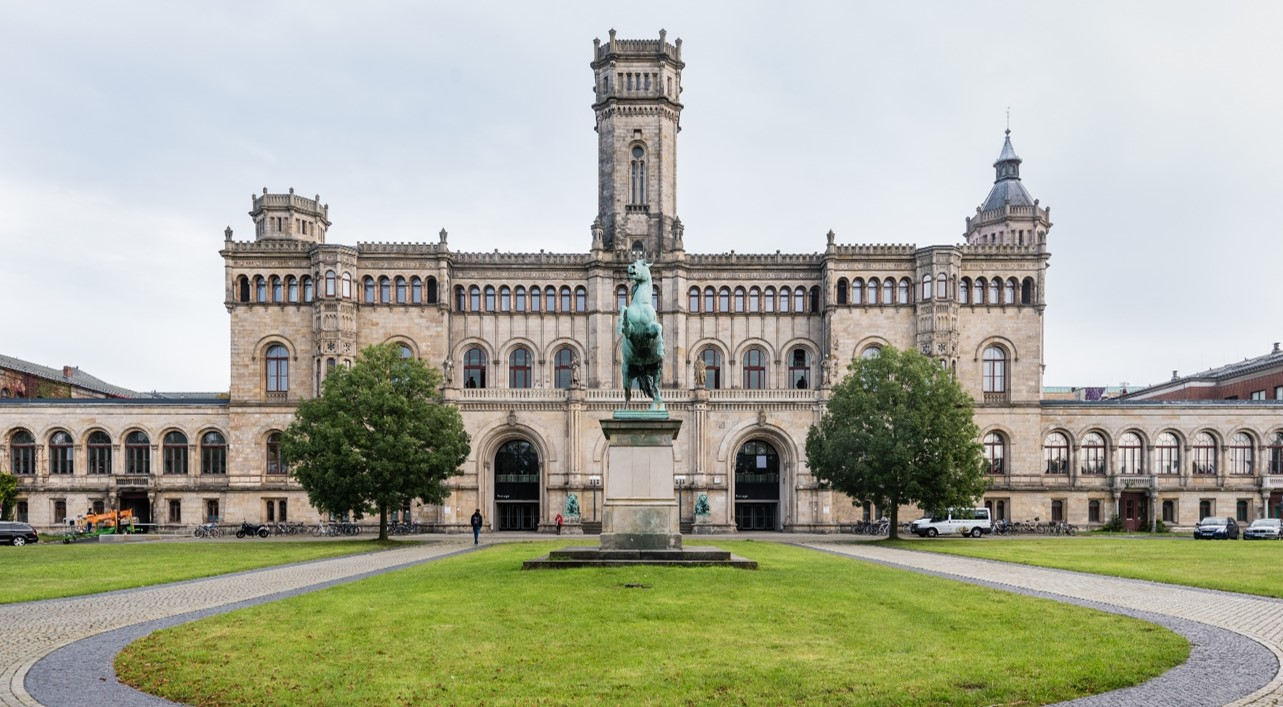
\includegraphics[width=0.65\textwidth]{figures/luh_default_presentation_title_image.jpg}}

% Title page: luhstyle
% \setbeamertemplate{title page}[luhstyle]
% % Add optional title image here
% \addtitlepageimage{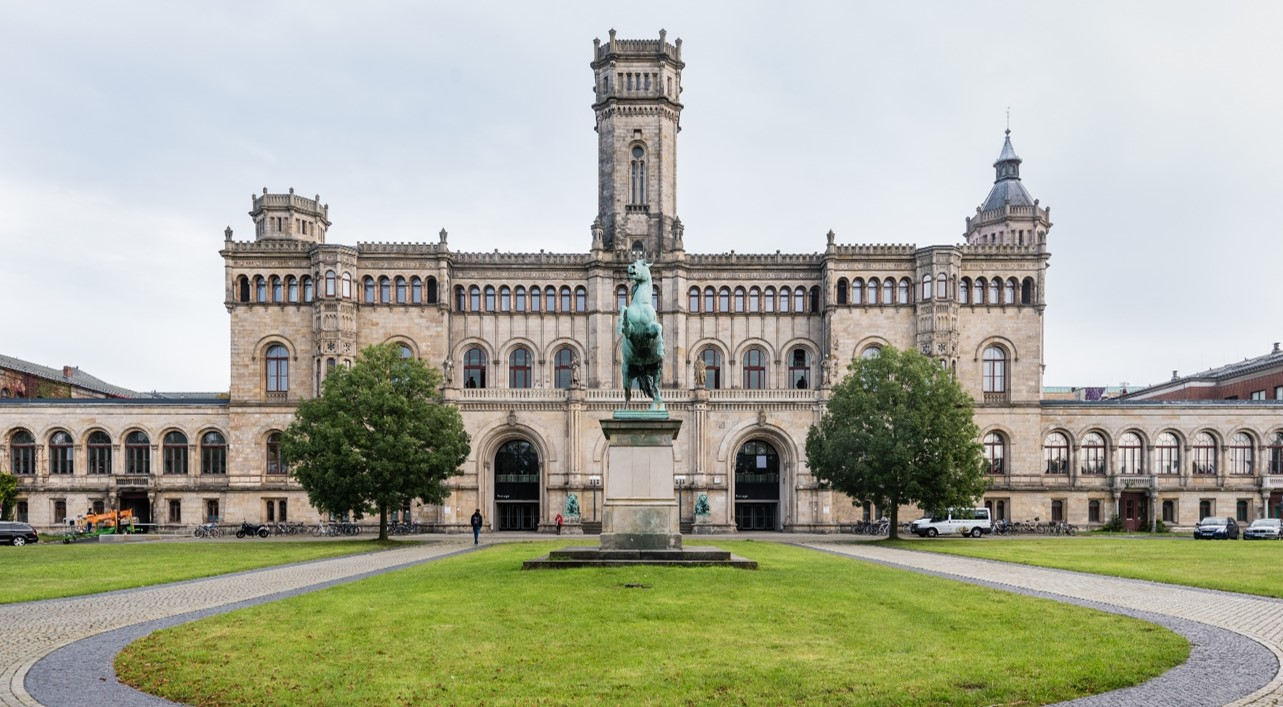
\includegraphics[width=0.75\textwidth]{figures/luh_default_presentation_title_image.jpg}}

\author[Abedjan \& Lindauer]{Ziawasch Abedjan \& Marius Lindauer\\[1em]
	
\includegraphics[height=\logoheight]{../latex_main/figures/luh_logo_rgb_0_80_155.pdf}\qquad
	
\includegraphics[height=\logoheight]{../latex_main/figures/DBIS_Kurzlogo.png}\qquad

\includegraphics[height=\logoheight]{../latex_main/figures/TNT_darkv4}\qquad

\includegraphics[height=\logoheight]{../latex_main/figures/L3S.jpg}	}
\date{Summer Term 2022; \hspace{0.5em} {
\includegraphics[height=1.5em]{../latex_main/figures/Cc-by-nc-sa_icon.svg.png}}; based on \href{https://ds100.org/fa21/}{[DS100]}
}


%%% Custom Packages
%----------------------------------------------------------------------
% Create dummy content
\usepackage{blindtext}

% Adds a frame with the current page layout. Just call \layout inside of a frame.
\usepackage{layout}


%%% Macros
%\renewcommand{\vec}[1]{\mathbf{#1}}
% \usepackage{bm}
%\let\vecb\bm

\title[Introduction]{DS: Clustering, Part 2}
\subtitle{Laplacian Matrix}

\graphicspath{ {./figure/} }
%\institute{}


\begin{document}
	
	\maketitle
	\begin{frame}{Dimensionality}
	    There is one problem with our adjacency matrix—it is very big!
	    \begin{itemize}
	        \item If our graph contains n vertices, its adjacency matrix will be of size $n^2$.
	        \item 10,000 vertices -> 100,000,000 entries in our matrix
	    \end{itemize}
	    \bigskip
	    We will need to reduce this matrix to fewer dimensions. How?
	    \\\bigskip
	    A: Eigenvalues and eigenvectors!\\
        However, we don’t want to use the adjacency matrix… see next slide. 
	\end{frame}
	
	
	
	\begin{frame}{Laplacian Matrix}
	    To reduce the dimensionality, we must first construct the Laplacian matrix L.
	    \begin{align*}
	        L=D-A
	    \end{align*}
	    D is a diagonal matrix, where each diagonal entry    $D_{ii}$     is equal to the sum of all of the edge weights connected to vertex i. All off-diagonal entries are 0. In math terms: 
	    \begin{align*}
	        &D_{ii}  =\sum\limits_{j=1}^nA_{ij}\\
	        &D_{ij}  = 0 \text{ if } i\neq j  
	    \end{align*}
	    (D actually contains the degree of each vertex, but we will not use this term.)
	\end{frame}
	
	
	
	\begin{frame}{Laplacian Matrix}
	    Here is the Laplacian matrix for our graph.\\
        Note that each row and each column sum to 0. It is also symmetric.\\
        A graph is also uniquely defined by its Laplacian matrix.

	    \begin{align*}
	        A = \left[\begin{array}{cccc}
	            0 & 5 & 3 & 1 \\
	            5 & 0 & 2 & 0 \\
	            3 & 2 & 0 & 0 \\
	            1 & 0 & 0 & 0
	        \end{array}\right] 
	        D = \left[\begin{array}{cccc}
	            9 & 0 & 0 & 0 \\
	            0 & 7 & 0 & 0 \\
	            0 & 0 & 5 & 0 \\
	            0 & 0 & 0 & 1
	        \end{array}\right] 
	        L = D-A =  \left[\begin{array}{cccc}
	            9 & -5 & -3 & -1 \\
	            -5 & 7 & -2 & 0 \\
	            -3 & -2 & 5 & 0 \\
	            -1 & 0 & 0 & 1
	        \end{array}\right] 
	    \end{align*}
	    \begin{figure}
	        \centering
	        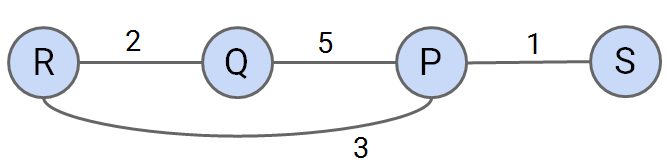
\includegraphics[scale=.5]{Bild15}
	    \end{figure}
	\end{frame}
	
	
	
	\begin{frame}{Eigenvectors of Laplacian}
	    Now, we determine the eigenvectors of the Laplacian matrix, and store them in a matrix V.\\
        The columns of V are sorted by their corresponding eigenvalue, in descending order.\\
        The corresponding eigenvalues here are 13.31, 7.44, 1.25, and 0.


	    \begin{align*}
	        V = \left[\begin{array}{cccc}
	            \vdots & \vdots &  & \vdots \\
	            v_1 & v_2 & \dots & v_n \\
	            \vdots & \vdots &  & \vdots
	        \end{array}\right] 
	        = \left[\begin{array}{cccc}
	            -.80 & .26 & -.22 & -.5 \\
	            .58 & .56 & -.31 & -.5 \\
	            .15 & -.78 & -.34 & -.5 \\
	            .06 & -.04 & .86 & -.5
	        \end{array}\right] 
	    \end{align*}
	    \begin{figure}
	        \centering
	        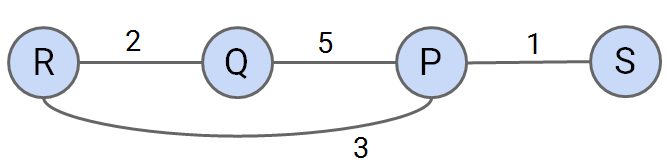
\includegraphics[scale=.5]{Bild15}
	    \end{figure}
	\end{frame}
\end{document}